\section{Zitierformate}
\label{sec:zitierformate}
In diesem Abschnitt wird auf unterschiedliche Zitierformate eingegangen, welche die Datenstruktur hinter einer Zitation beschreiben.
In dieser Arbeit wird sich auf das \gls{cff} und das \hologo{BibTeX}-Format beschränkt.
Das \gls{cff} ist ein Format, welches speziell für die Zitation von Software entwickelt wurde, weshalb es in dieser Arbeit besonders interessant ist.
Das \hologo{BibTeX}-Format wird dazu verwendet, um zumeist in Verbindung mit \LaTeX{}, Bibliographien zu erstellen und ist daher ebenfalls von Interesse, da es auch für Software verwendet werden kann.

\subsection{Citation File Format}
\label{subsec:citation-file-format}
Das \gls{cff} ist ein Format, welches in der \mintinline{text}{CITATION.cff}-Datei gespeichert wird und in YAML 1.2 geschrieben wird. 
Das Format beschreibt die Zitation von Software und kann von Menschen und Maschinen gelesen werden.
Es enthält Metadaten, welche für die Zitation von Software benötigt werden.
Außerdem wird es öffentlich auf GitHub verwaltet.
Auf GitHub enthalten 2.512 Repositorys eine \mintinline{text}{CITATION.cff}-Datei (Stand 07.11.2024).
Softwareentwickler können das \gls{cff} in ihre Repositorys einbinden, um anderen die Zitation ihrer Software zu erleichtern und vorzugeben, wie die Software richtig zu zitieren ist \autocite{druskat_citation_2021}.

Da die Datei von Menschen gelesen werden kann, kann diese manuell erstellt werden und in das Repository eingebunden werden.
Die Spezifikationen für das \gls{cff} werden auf GitHub verwaltet und sind öffentlich einsehbar \autocite{druskat_citation_2021}.
Ebenfalls existieren Programme, welche das \gls{cff} verarbeiten können.
Beispielsweise kann das Programm \emph{cffinit} genutzt werden, um eine \mintinline{text}{CITATION.cff}-Datei zu erstellen, sodass der Prozess der Erstellung vereinfacht wird \autocite{spaaks_cffinit_2023}.
Ein weiteres Beispiel ist das Programm \emph{cffconvert}, welches das \gls{cff} in verschiedene Formate umwandeln kann, wie z.~B. \hologo{BibTeX} oder RIS.
Außerdem kann das Programm genutzt werden, um \gls{cff}-Dateien zu validieren \autocite{spaaks_cffconvert_2021}.

Zusätzlich wird das \gls{cff} von unterschiedlichen Plattformen unterstützt, wie z.~B. von GitHub.
Erkennt GitHub eine \mintinline{text}{CITATION.cff}-Datei im Repository auf dem Standardbranch, wird sie automatisch auf der Repository-Startseite verlinkt und kann direkt im \hologo{BibTeX}-Format kopiert werden \autocites{druskat_citation_2021}{github_about_2024-1}.
Ebenfalls ist es möglich, die in der Datei eingetragenen Autoren in der APA-Zitierweise zu kopieren.
Die Funktionen sind in \autoref{fig:gh_cff_link} dargestellt.

\begin{figure}
    \begin{center}
      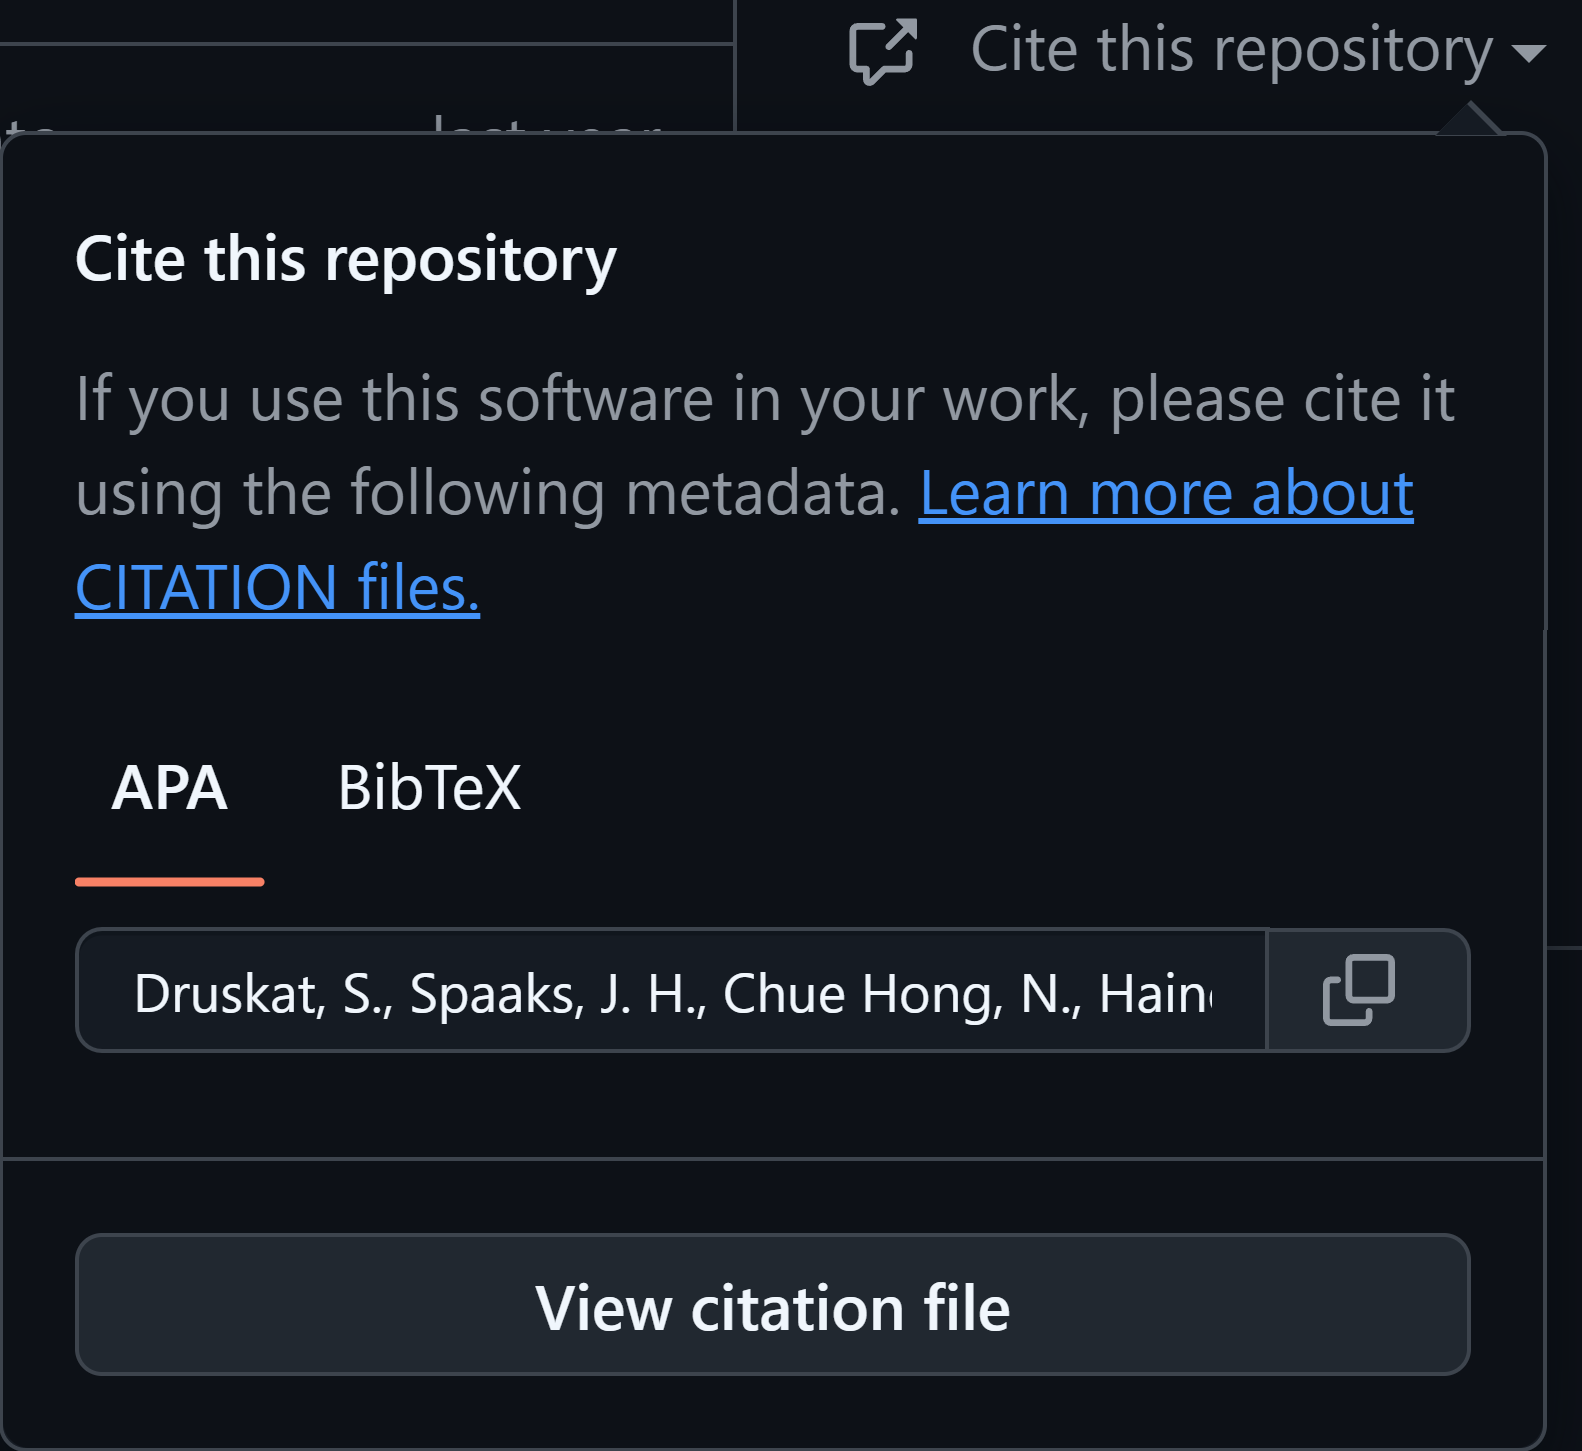
\includegraphics[width=0.5\textwidth]{bilder/GH_CFF_link.png}
    \end{center}
    \caption{GitHub-Repository mit \mintinline{text}{CITATION.cff}-Datei}
    \label{fig:gh_cff_link}
    \small
    Die Abbildung stellt den Link auf die \mintinline{text}{CITATION.cff}-Datei dar, wie ihn GitHub aktuell darstellt.
    Außerdem ist die Möglichkeit sichtbar, die Datei im \hologo{BibTeX}-Format und in der APA-Zitierweise zu kopieren \autocite{druskat_citation_2021-1}.
\end{figure}

In dem \gls{cff} existieren verschiedene Felder, welche für die Zitation von Software relevant sind.
Das wichtigste Feld ist das \emph{authors}-Feld, welches die Autoren der Software enthält und zwingend erforderlich ist.
In diesem Feld können die Autoren als Liste angegeben werden.
Ein Autor ist dabei entweder eine Person oder eine Entität.
Eine Entität kann beispielsweise eine Organisation sein.
Die Entität kann mit einem Namen mittels \emph{name} angegeben werden \autocite{druskat_citation_2021}.
Sie kann ebenfalls eine OORCID iD und eine E-Mail-Adresse enthalten.
Besonders wichtig für diese Arbeit ist die Referenz auf eine Person, da dies die einzige Information ist, welche aus Git extrahiert werden kann.
Eine Person enthält ebenfalls die genannten Werte einer Entität und wird jedoch über den Vor- und Nachname separiert mittels \emph{given-names} und \emph{family-names} angegeben.
Dadurch ist es möglich, die Personen von den Entitäten zu unterscheiden.

Ein weiteres Feld ist das \emph{preferred-citation}-Feld.
Mit diesem Feld ist es möglich, die Anerkennung für die Arbeit auf eine andere Arbeit zu übertragen \autocite{druskat_citation_2021}.
Ein Beispiel hierfür ist ein Paper über die Software, welches bevorzugt zitiert werden soll, anstelle der eigentlichen Software.
Hierbei können ebenfalls Personen und Entitäten angegeben werden.
Durch die Angabe einer \emph{preferred-citation} kann das Prinzip der Wichtigkeit vernachlässigt werden.
Auf dieses Verhalten wird in der Diskussion konkreter eingegangen.

Weitere in dieser Arbeit verwendete Felder sind \emph{type}, \emph{year}, \emph{month}, \emph{date-released}, \emph{date-published}, \emph{doi}, \emph{collection-doi} und \emph{identifiers}.
Das Feld \emph{type} ist zwingend erforderlich, hat jedoch als Standardwert \glqq software\grqq{}, sodass dies nicht angegeben werden muss.
Es gibt an, ob es sich um eine Software oder einen Datensatz handelt.
Dabei sind lediglich die Werte \glqq software\grqq{} oder \glqq dataset\grqq{} erlaubt.
Das Feld \emph{date-released} gibt an, wann die Software oder der Datensatz veröffentlicht wurde.
Das Feld \emph{doi} kann einen \glspl{doi} der Software oder des Datensatzes enthalten.
Mittels \emph{identifiers} können weitere Identifikatoren angeführt werden, wie z.~B. eine \gls{doi} oder eine URL, wobei die \emph{identifiers} mit einer Beschreibung erweitert werden können.
Die beschriebenen Felder können zusätzlich alle unter dem Feld \emph{preferred-citation} angegeben werden, um eine andere Arbeit zu referenzieren.

Die Felder \emph{year}, \emph{month} und \emph{date-published} können zusätzlich zu dem Feld \emph{date-released} unter dem Feld \emph{preferred-citation} angeführt werden, um das Jahr und das Datum der Veröffentlichung anzugeben.
Außerdem können weitere Typen mittels \emph{type} aufgeführt werden, wie beispielsweise \glqq thesis\grqq{} oder \glqq manual\grqq{}, sodass diese Arbeiten ebenfalls referenziert werden können.
Zusätzlich kann das Feld \emph{collection-doi} verwendet werden, um auf eine Sammlung von Arbeiten zu verweisen, die die Arbeit enthält.
Ein Beispiel einer \mintinline{text}{CITATION.cff}-Datei ist in \autoref{lst:cff_example} dargestellt.
Dabei wurde sich auf die beschriebenen und notwendigen Felder beschränkt.

\begin{listing}
    \inputminted{yaml}{../CITATION.cff}
    \caption{Beispiel einer \mintinline{text}{CITATION.cff}-Datei}
    \label{lst:cff_example}
    \small
    In dem Listing ist die \gls{cff}-Datei dieser Arbeit dargestellt. Dabei wurden primär Felder angegeben, welche in der Masterarbeit verwendet werden.
\end{listing}

\subsection{\hologo{BibTeX}}
\label{subsec:bibtex_format}
\hologo{BibTeX} ist eine Software, welche zur Erstellung von Literaturangaben und -verzeichnissen in \LaTeX{}-Dokumenten verwendet wird.
Außerdem existiert mit \hologo{BibTeX} ein gleichnamiges Format, welches in der \mintinline{text}{CITATION.bib}-Datei gespeichert wird und auf keinem anderen Format basiert.
\hologo{BibTeX} ist ein weit verbreiteter Standard und wird von vielen Autoren in der Wissenschaft verwendet.
Auf GitHub enthalten 2.144 Repositorys eine \mintinline{text}{CITATION.bib}-Datei (Stand 07.11.2024).
Das Format beschreibt die Zitation von Literatur und kann von Menschen und Maschinen gelesen werden.
Es beschränkt sich dabei nicht auf eine spezielle Art von Literatur, sondern kann für viele unterschiedliche Arten von Literatur verwendet werden.
Beispielsweise können Bücher und Masterarbeiten in \hologo{BibTeX} zitiert werden \autocite{patashnik_bibtexing_1988}.
Ein offizieller Literaturtyp für Software existiert nicht.
In der Datei können mehrere Einträge vorhanden sein, wobei jeder Eintrag eine Literaturangabe darstellt.

\hologo{BibTeX}-Dateien können von Menschen manuell erstellt und in das Repository eingebunden werden.
Außerdem existieren viele Literaturverwaltungsprogramme wie Zotero, welche \hologo{BibTeX}-Dateien erstellen und verarbeiten können \autocite{zotero_zotero_2024}.
Ebenfalls ist die Integration in andere Plattformen möglich, wie z.~B. in GitHub.
Hier wird die \mintinline{text}{CITATION.bib}-Datei auf der Repository-Startseite verlinkt, sie lässt sich jedoch im Gegensatz zu dem \gls{cff} nicht direkt kopieren oder in andere Formate umwandeln \autocite{github_about_2024-1}.

In dem \hologo{BibTeX}-Format existieren verschiedene Felder, welche für die Zitation von Literatur relevant sind.
Welche Felder zwingend erforderlich sind, hängt vom jeweiligen Literaturtyp ab, während andere optional bleiben.
Zudem sind die verfügbaren Felder ebenfalls vom Literaturtyp abhängig \autocite{patashnik_bibtexing_1988}.
In dieser Arbeit wird auf einige dieser Felder eingegangen, welche für die spätere Auswertung relevant sind.
Das wichtigste Feld ist das \emph{author}-Feld, welches die Autoren der Literatur enthält und zwingend erforderlich ist.
Die Vor- und Nachnamen der Autoren werden mit einem Komma separiert und mehrere Autoren werden über ein \glqq and\grqq{} getrennt.
Weitere Felder, welche für die Masterarbeit verwendet werden, sind \emph{year} und \emph{month}, welche das Jahr und den Monat der Veröffentlichung angeben.
Ein Beispiel einer \mintinline{text}{CITATION.bib}-Datei ist in \autoref{lst:bibtex_example} dargestellt.
Es ist zu erkennen, dass in dem \hologo{BibTeX}-Eintrag Informationen fehlen, welche in dem \gls{cff}-Eintrag vorhanden waren.
Dies liegt daran, dass in dem \hologo{BibTeX}-Eintrag nur eine Referenz auf die Masterarbeit möglich ist und nicht auf die entwickelte Software.

\begin{listing}
  \inputminted{text}{../CITATION.bib}
  \caption{Beispiel einer \mintinline{text}{CITATION.bib}-Datei}
  \label{lst:bibtex_example}
  \small
  In dem Listing ist die \hologo{BibTeX}-Datei dieser Arbeit dargestellt. Dabei wurden primär Felder angegeben, welche in der Masterarbeit verwendet werden.
\end{listing}
